\documentclass[en]{jdoc}
\include{macros-ph}
\usepackage{bm}
\usepackage{graphicx}
\usepackage{caption}
\usepackage{subcaption}

\usepackage{tikz}
\usetikzlibrary{fit}
\usetikzlibrary{arrows}
\usetikzlibrary{positioning}
\usepackage{stmaryrd}


\ed{PRES LUNAM \\ École Doctorale STIM \\ Sciences et Technologies de l'Information
et Mathématiques}
\spec{BioInformatics}
\labo{IRCCyN}
\equipe{MeForBio}
\title{Qualitative Modeling of Gene Regulatory Networks}
\author{Courtney Chancellor}
\email{Courtney.Chancellor@ec-nantes.fr}


\begin{document}

\makehead
 
 \begin{abstract}
 Our ability to gather data in the context of gene regulatory networks has skyrocketed in the past decades, 
the scale of which is massive and uninterpretable without applying formal analysis. Qualitative modeling techniques are commonly used in this context as they are able to scale up with large, interconnected graphs with high degrees of abstraction. Analysis, however, may be limited to the questions and tools which do not require the construction of the full state space, which grows exponentially. By addressing these models with numerical tools capable of solving high-dimensional problems, we are able to directly access the probability of the system occupying any state at any given time. For this work, we have successfully implemented Proper Generalized Decomposition
\end{abstract}

\begin{keywords}
 genetic regulation, 
 qualitative modeling, 
 high dimensional systems, 
 numerical methods
\end{keywords}

\begin{collaborations}
Francisco Chinesta,
Morgan Magnin,
Olivier Roux
\end{collaborations}

\section{Introduction}

  A large part of bioinformatics is dedicated to the modeling of biological systems with the hopes of supplementing experimental work or informing experimental design. Many modeling frameworks exist, each of which brings its own strengths and weaknesses, data requirements and fundamental assumptions. As a result, what kind of framework to choose is largely informed by the characteristics of the system or the nature of the information we wish to derive from our model. For regulation of genetic expression, qualitative modeling schemes can be advantageous as they are well suited for handling the very large, interconnected graph of interacting species typical of these systems. However, in exchange for being scalable, qualitative models typically give limited access to the underlying probability distribution of the state space, normally requiring simulation techniques. In our work, we attempt to apply numerical methods to qualitative systems in order to directly access this probability distribution, deepening our potential to analyze very large, or high dimensional, systems. We begin by taking a Process Hitting model, a qualitative modeling framework which demonstrates excellent scalability and possesses several efficient analysis tools. By using Proper Generalized Decomposition, we are able to access a full solution space given an initial condition without simulation.
  
  \section{Qualitative Models and Process Hitting}
  
  In our work, we are given an initial description of a biological system such as ``gene A activates gene B after passing some threshold value.'' This is quite different than kinetic models, which generally demonstrate mass action rate laws: ``two molecules of A combine with one molecule of B to produce C at rate r'', which are treated with quantitative frameworks. The network of influence between genes is called the \textit{regulatory network} and is commonly represented as a directed, signed graph. Qualitative frameworks attempt to use this information to construct functional models of a given system in order to perform in-depth analysis or \textit{in silico} experiments. Process Hitting is one of many possible qualitative approaches. This technique abstractly represents all participating elements of a network, albeit genes, proteins or environmental factors, as automata. These automata possess local states (on/off, low/medium/high concentrations, etc) which interact with one another to move the system from one state to another. Such interactions are divided into two parts, the initial influence and the resulting transition. The translation of a directed graph to Process Hitting can be found in Figure \ref{PH_fig}.
   \begin{figure}[h]
\begin{subfigure}[t]{0.3\textwidth}
   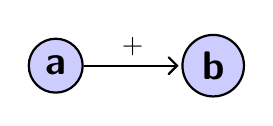
\begin{tikzpicture}[->,>=stealth',shorten >=1pt,auto,node distance=2cm,
  thick,main node/.style={circle,fill=blue!20,draw,font=\sffamily\Large\bfseries}]
  \node[main node] (a) {a};
  \node[main node] (b) [right of=a] {b};
  \path[->,>=angle 90]
(a) edge node[above]{$+$} (b);
\end{tikzpicture}
\end{subfigure}
\begin{subfigure}[b]{0.35\textwidth}
\resizebox{.9\textwidth}{!}{
 \begin{tikzpicture}[scale=2]
  \draw (-1,0) rectangle (1,1);
  \node [rotate=90] at (-1.25,.5) {\% of effect};
    \node [bottom] at (0,-.25) {concentration of activator};

  \draw [red] (0,0) -- (0,1);
    \foreach \x in {-1,-0.75,...,1}{
      \draw[y=1cm,thick,blue] (\x,0) -- (\x,-0.1);
      ;
    }
    \foreach \y in {0.5,1}{
      \draw[thick,blue] (0,\y) -- (-0.2,\y);
      \node at (-0.45,\y) {\y};
    }
    \coordinate (a) at (1,1);
    \coordinate (b) at (-1,0);
    \draw (b) edge[ultra thick,out=360,in=180,looseness = 2.25] (a);    
  \end{tikzpicture}}
  \end{subfigure}
\begin{subfigure}[b]{0.33\textwidth}
\begin{tikzpicture}
\TSort{(0,0)}{a}{2}{l}
\TSort{(2,0)}{b}{2}{r}
\THit{a_1}{}{b_0}{.west}{b_1}
\path[bounce, bend left]
\TBounce{b_0}{}{b_1}{.south};
\end{tikzpicture}
\end{subfigure}

\caption{Creating a Process Hitting action. In gene regulation, we consider two kinds of interactions between species: activation and inhibition. If $a$ is an activator of $b$, it is common to represent this by a signed, directed graph (left). These interactions have a characteristic form: unlike kinetic reactions, activation and inhibition usually depend on the regulator passing some threshold concentration in order to become effective (middle). Process Hitting (right) represents these reactions via actions: $a$ activates $b$ becomes $a_1$ interacts with $b_0$ to make it transition (bashed arc) to $b_1$. Every action can be associated with temporal and stochastic parameters-- the reaction rate, for example.}
\label{PH_fig}
\end{figure}
Although this is a highly abstract representation of a biological process, Process Hitting semantics allow us to easily model interactions with only partial knowledge of the system as a whole. For example, it is sufficient to know that one gene inhibits another, without knowing the exact mechanism therein. Furthermore, Process Hitting possesses powerful static analysis techniques in order to study steady state behavior, the reachability of a certain state from another, and cut sets which determine minimum criteria for reachability, all of which are done without the need of constructing the full state space, making it a very scalable framework. Models of up to 10,000 interacting species \cite{} have been successfully addressed using Process Hitting. However, this analysis is somewhat limited in scope. To answer deeper, more nuanced questions of the model, we must be able to access the full solution space, the probability of the system existing at any state,$z$ at a given time, $t$, or $\Phi(z,t)$. This probability distribution can be accessed via the Markov Jump Equations of the model which track the possible transitions between states through time. While using these equations for simulation have been historically prevalent, the application of numerical techniques has the potential to do the same but without computationally prohibitive trial runs.
\section{Numerical Technique: Proper Generalized Decomposition}
Proper Generalized Decomposition is a reduced basis technique which assumes that the target, in this case, the probability distribution, can be written as a sum of a product of separable functions of the interacting species, $F(z_i)$ $i=\{1\cdots N_{sp}\}$, and time, $F(t)$:
\[
 \Phi(z,t)\cong \sum_{j=1}^{M}F_1^j(z_1)\cdots F_2^j(z_2)\cdots F_{N_{sp}}^j(z_{N_{sp}}) \cdot F_t(t)
\]
PGD is performed iteratively, starting at some arbitrary guess and searching for sets of functions, one vector at a time, which will minimize the residual of the running sum. Although the accuracy increases with every addition, we assume that only a limited number, $M$, of sets of functions are needed to capture the behavior of the system. We have not changed the state space but, rather, re-ordered it such that only one $N\times1$ vector, usually on the scale of 2 or 3 since this size represents the possible local states of a qualitative model, must be addressed at any given time, see Figure \ref{cubes}. All operations can be performed by canonical techniques and are highly parallelizable, therefore iterations are generally fast and computationally inexpensive.
\begin{figure}[h]
\centering
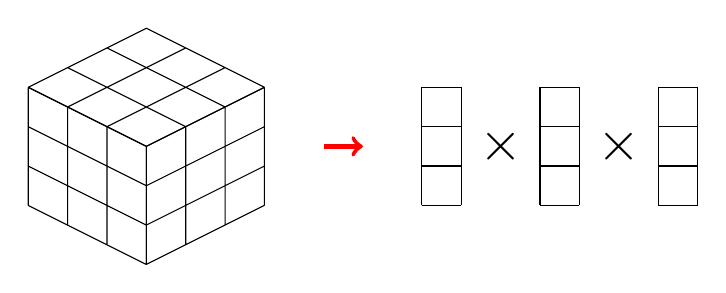
\begin{tikzpicture}[scale=0.5]

  \draw[yslant=-0.5] (0,0) grid (3,3);

  \draw[yslant=0.5] (3,-3) grid (6,0);
  \draw[yslant=0.5,xslant=-1] (3,0) grid (6,3);
  
  \draw [->,red,ultra thick] (7.5,1.5) -- (8.5,1.5);
  \draw (10,0) grid (11,3);
  \node[scale=2] at (12,1.5) {$\times$};
  \draw (13,0) grid (14,3);
    \node[scale=2] at (15,1.5) {$\times$};
  \draw (16,0) grid (17,3);
\end{tikzpicture}
\caption{Decomposition of a state space. This illustration shows how a multidimensional space, for example, a cubic space of three dimensions, $3^3$ can be decomposed into the product of the individual dimensions, $3\times 3$. This mathematical property is exploited by PGD in that we search for sets of $N_{sp}$ $(1\times N)$ vectors  which are relatively small compared to the full $N_{sp}^N$ state space. Repeated $M$ times such that each new set minimizes the residual, the results are summed to produce the final approximation.}
\label{cubes}
\end{figure}

\section{Application on a Example Toy Model}
\begin{figure}[h!]
\centering
 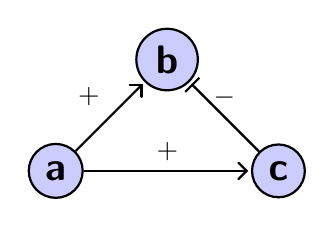
\begin{tikzpicture}[->,>=stealth',shorten >=1pt,auto,node distance=2cm,
  thick,main node/.style={circle,fill=blue!20,draw,font=\sffamily\Large\bfseries}]
  \node[main node] (1) {a};
  \node[main node] (2) [above right of=1] {b};
  \node[main node] (3) [below right of=2] {c};
  \path[->,>=angle 90]
(1) edge node[above left]{$+$} (2)
(1) edge node[above]{$+$}(3);
\path[-|](3) edge node[above]{$-$} (2);
\end{tikzpicture}

  \caption{\label{toy}The toy network developed for this overview, an incoherent feed forward loop, ``incoherent'' as A both directly activates B and indirectly inhibits B via C.}

\end{figure}
\end{document}
